\section{Einleitung}

Die bipedalen Bewegungsformen des Menschen, Gehen und Laufen, sind durch ein komplexes Zusammenspiel von neuronalen, physiologischen und mechanischen Prozessen gekennzeichnet. 
Das Gangbild unterscheidet sich von Mensch zu Mensch, abhängig von Parametern wie Alter, Körpergröße, Gewicht, Schuhwerk und physischer Verfassung (Görz-Neumann 2016). 
Ein Schrittzyklus bezeichnet den sich wiederholenden Vorgang, des Beinhebens, -schwingens, dem Aufsetzen und Belasten. Dieser Zyklus wird in acht Phasen unterteilt, abgebildet in \autoref{fig:Skizze_Phasen} und näher beschrieben in (Perry 2003). Modellhaft kann man sich den Schrittzyklus auch als zwei Pendelbewegungen vorstellen: Während der Standphasen pendelt die Hüfte um den Standmittelpunkt, während der Schwungphasen pendelt das Bein um die Aufhängung in der Hüfte. Ersteres wird auch als Inverses-Pendel-Modell bezeichnet.
Wenn sowohl das linke als auch das rechte Bein einen Schrittzyklus durchgeführt haben spricht man von einem Doppelschritt und der Körper befindet sich wieder in der Ausgangslage.\\
Diese Modelle erlauben den Vergleich des Gangbildes mit einem mathematischen Pendel. Die Eigenfrequenz eines Pendelsystems ist dabei diejenige, welche sich ohne äußere Kraftwirkung allein aus der Erdbeschleunigung und der Pendellänge, also dem Abstand des Punktmasse zur Pendelaufhängung, ergibt. Dieser Abstand wird für das Modell jeweils als derjenige zwischen Rotationsmittelpunkt und Massenzentrum der rotierenden Masse bestimmt.\\
Für verschiedene Aufgabenstellungen ergeben sich verschiedene Gangstile, die beispielsweise das optimale Strecken zu Energieverbrauch Verhältnis aufweisen oder besonders Energie pro Zeit effizient sind.\\
\begin{figure}[h!]
	\centering
	\includegraphics[width=\linewidth]{bilder/Einleitung/Skizze_Gangphasen_small}
	\caption[Gangphasen]{Unterteilung des Schrittzyklus in acht Phasen: vier Phasen des Standes, vier Phasen des Schwingens.}
	\label{fig:Skizze_Phasen}
\end{figure}

Für ein vollständiges Verständnis der Prozesse, welche beim Gehen ablaufen sind neben der rein mechanischen Betrachtung, auch physiologische und Neurologische Fragen zu bearbeiten. Der vorliegende Bericht soll sich jedoch allein mit der biomechanischen Untersuchung des Gehens befassen. \\
Diese lässt sich unterteilen in die Aspekte Kinematik und Kinetik. Die Kinematik ist dabei die Beschreibung der Bewegung von Gelenken und Segmenten im Raum, die Kinetik befasst sich mit der Beschreibung von Kräften und Momenten, die während der Lokomotion auftreten (WINTER 2009). Auf einem Laufband lässt sich die zyklische Natur der Bewegungsabläufe studieren, da es zu keiner realen Ortsänderung kommt. Hier sollen die kinematischen Aspekte des Gehens untersucht werden. \\
Weiterhin sollen die während der Standphase auftretenden Kräfte mit der Methode der inversen Dynamik untersucht werden. Hierfür wird ein zweites Experiment durchgeführt, wobei der Proband über eine Laufstrecke mit eingebauter Waage, welche Bodenreaktionskräfte aufnimmt, läuft. Es ist so möglich, die Kräfte, welche in den Gelenken des Beines auftreten, durch Aufstellen von Kräftegleichgewichten zu bestimmen.
Voraussetzungen für diese Beschreibungen sind gewisse Annahmen, welche im Folgenden aufgeführt sind:\\
\begin{itemize}
\item Jedem Segment, d.h. der Abschnitt zwischen zwei Gelenken, werden eine konstante Masse in einem unbeweglichen Schwerpunkt, ein konstantes Trägheitsmoment und eine fixierte Länge zugewiesen.
\item Alle Gelenke werden als rein rotative Gelenke (Scharniere) betrachtet
\item Die Position der Gelenke wird von außen abgeschätzt
\item Die Position der Abschnittsschwerpunkte und die Masse der Abschnitte wird durch Anthroprometrietabellen bestimmt
\end{itemize}
Beispielhaft sind in \autoref{fig:experimente} zwei Bilder aus den durchgeführten Experimenten zu sehen. Farbig eingezeichnet sind die Trajektorien der Gelenkmarker.
\begin{figure}
	\centering
	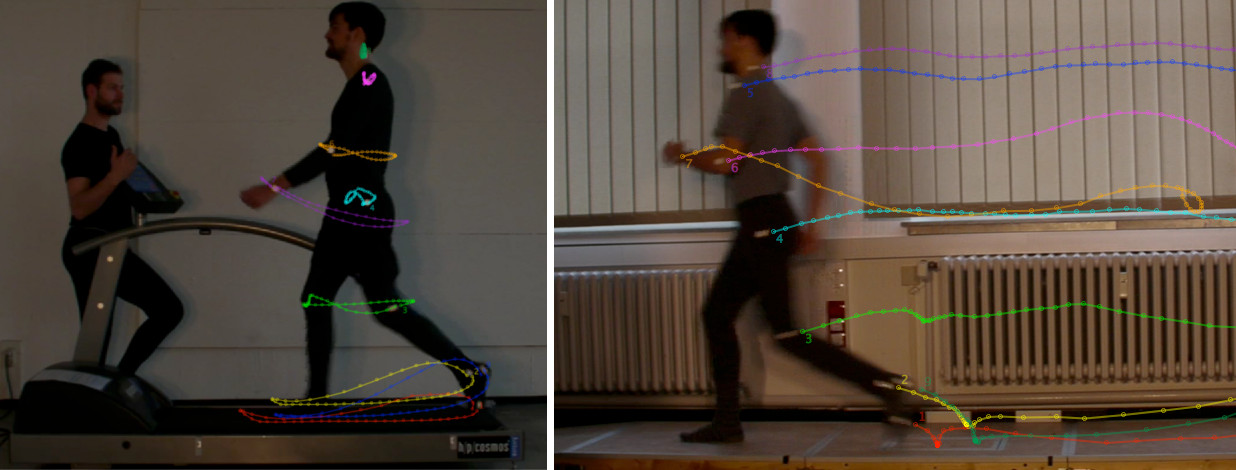
\includegraphics[width=\linewidth]{bilder/Einleitung/lauf_experimente.jpg}
	\caption[Experimente]{Links: Aufnahme aus dem Laufbandversuch mit getrackten Markern. Rechts: Aufnahme aus dem Laufstegversuch mit getrackten Markern.}
	\label{fig:experimente}
\end{figure}



%Der bipedale Gang des Menschen ist ein Erkennungsmerkmal unserer Fortbewegung und weist ein Alleinstellungsmerkmal gegenüber anderer bipedalen Bewegungsstilen auf: die fast vollständige Streckung der Beine (ALEXANDER 1992). Die Erforschung der menschlichen Fortbewegung erstreckt sich dabei von der Ganganalyse (alexander und wer noch so alles) über klinische Forschung (WREN ET AL 2011) bis hin zur Untersuchung von Laufmustern für Roboter (TLOK-XXX und ...noch eins..).
%Um den Gang genauer zu untersuchen wird der Gangzyklus grundlegend unterteilt in Standphase und Schwungphase sowie weitere Sub-Phasen, die in Abbildung \ref{fig:Skizze_Phasen} dargestellt sind (Perry XXX).\\
%Der Menschliche Gang lässt sich dabei sehr gut mit dem Modell eines inversen Pendels abstrahieren. Durch das fast vollständig gestreckte Standbein rotiert die Hüfte um den Kontaktpunkt mit dem Boden. Das Schwungbein verhält sich dagegen wie ein normales Pendel und schwingt um die Hüfte. Mit der Distanz des Beinschwerpunktes bis zur Hüfte lässt sich das Bein als mathematisches Pendel abstrahieren und so die Eigenfrequenz des Beines bestimmen. Bewegt man sich mit der Geschwindigkeit fort, bei der das jeweilige Schwungbein mit dieser Periodendauer schwingt, ist für die Beinbewegung keinerlei Energie notwendig (KUO 2007, HIER VLLT ANDERE QUELLE?!?!).\\

%Das Modell des inversen Pendels kann durch den subjektiven Energieaufwand beim Gehen überprüft werden. Bewegt man sich mit genau der richtigen Geschwindigkeit fort, sollte das Laufen als sehr angenehm empfunden werden und ohne großen Kraftaufwand möglich sein.
%\begin{wrapfigure}{r}{6cm}
%	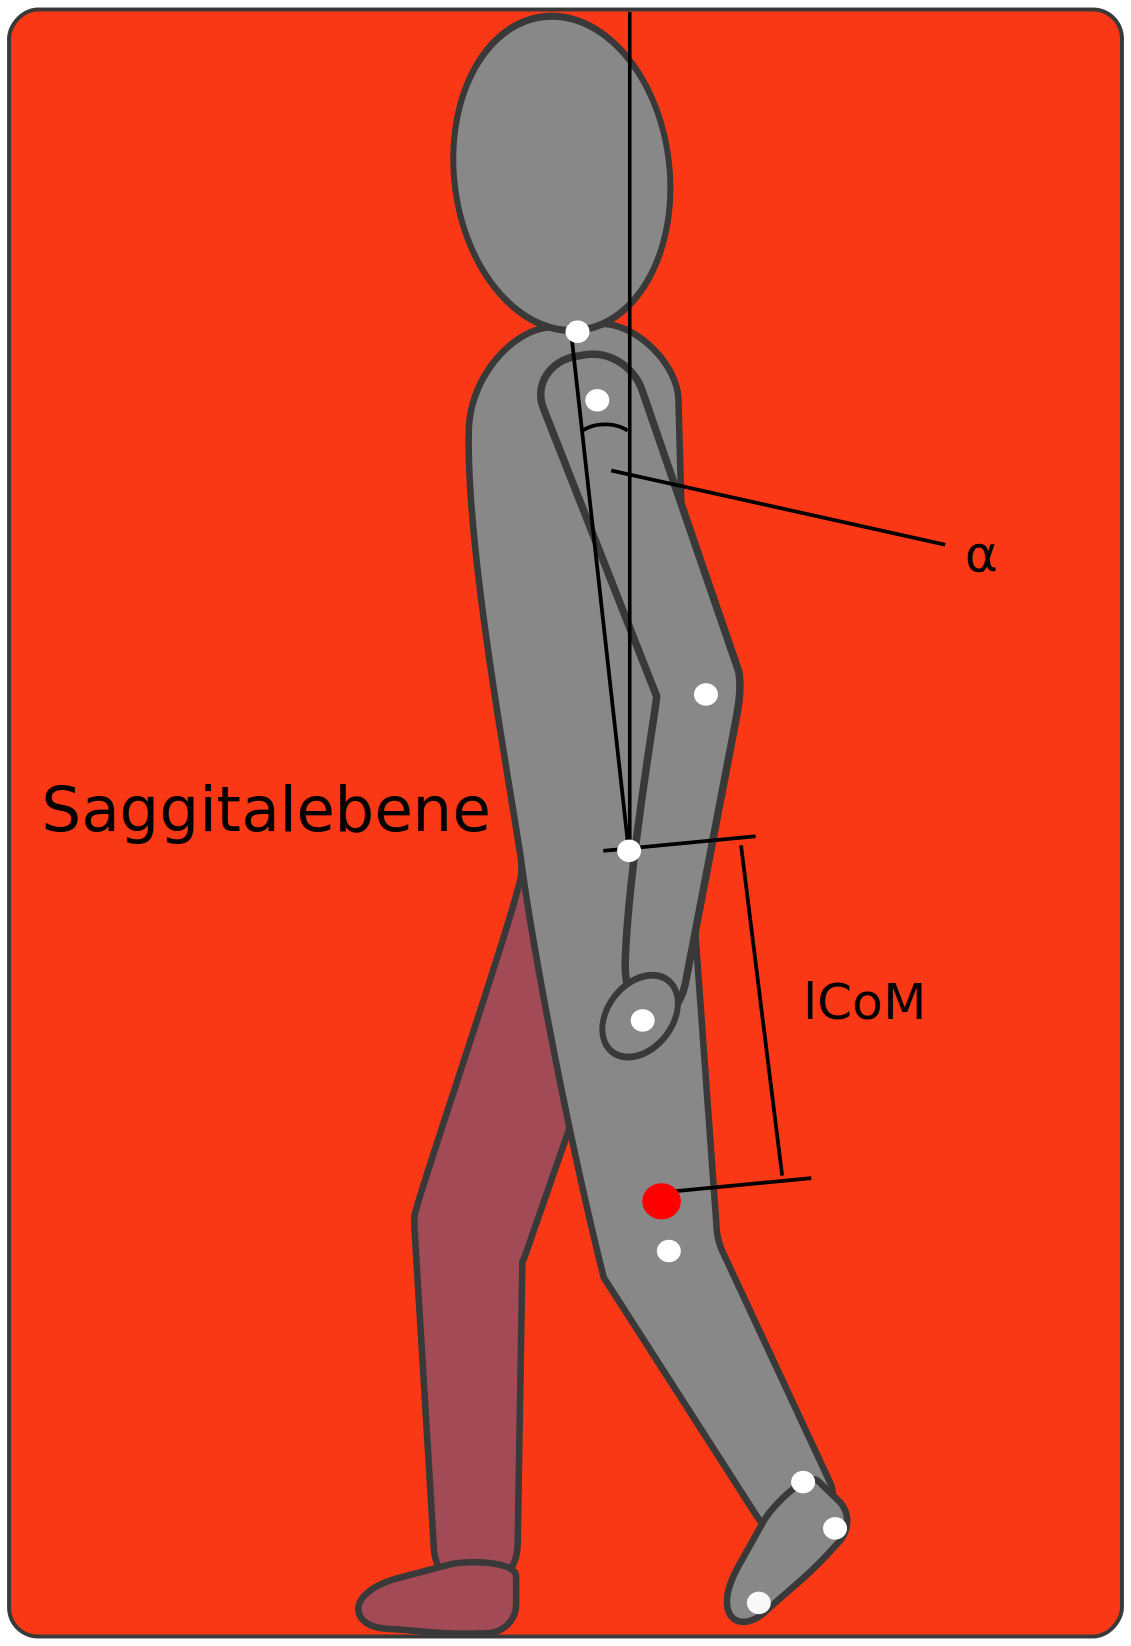
\includegraphics[width=\linewidth]{bilder/Einleitung/Proband_Pendel}
%	\caption[Inverses Pendel und untersuchte Gelenke]{Untersuchungsebene, wichtige Gelenke (weiße Kreise), Länge des virtuellen Pendels ($l_{CoM}$) von Hüfte bis zum Massenschwerpunkt des Beines (roter Kreis) sowie Neigungswinkel des Oberkörpers zur Senkrechten ($\alpha$)}
%	\label{fig:Proband_Pendel}
%\end{wrapfigure}
%Weitere Aussagen über den Gang lassen sich durch das Messen der Bodenreaktionskräfte (BRK) treffen. Verbindet man diese mit der kinematischen Analyse können Momente wie Lastaufnahme in Y-Richtung sowie ein Abbremsen und Abstoßen in X-Richtung beobachtet werden. Die Kräfte in Z-Richtung erlauben Aussagen über die Balance beim Gehen, welche besonders interessant sind für die monopedalen Stützphasen (ehhh, QUELLE?).
%Ziel dieser Arbeit ist die exemplarische Datenerhebung mittels kinematischer und kinetischer Verfahren für einen Probanden. Das Gehen wird bei verschiedenen Geschwindigkeiten untersucht und eine allgemeine Auswertung von Periodendauer durchgeführt, um die Theorie des inversen Pendels zu testen. Die Versuche auf dem Laufband und der Laufstrecke werden auf Unterschiede in der Körperneigung und der Handtrajektorie verglichen. Unterschiede zwischen den beiden Experimenten könnten auf eine Anpassung des Gehens an die tatsächliche Ortsänderung auf der Laufstrecke sein. Zusammen mit den Kraftmessungen werden mittels inverser Kinematik auf der Laufstrecke die auftretenden Kräfte und Momente in Knöchel, Knie und Hüfte untersucht und hier Aussagen zu ( JA ZU WAS DENN?? LAUFROBOTER??, BESSERE SCHUHE??) abgeleitet. Alle ermittelten Daten werden mit der Literatur verglichen und die Experimente auf ihre Belastbarkeit geprüft, da auf eine statistische Belastabrkeit der Messdaten verzichtet wurde, um den Umfang der Untersuchungen zu erhöhen.\\







%\begin{figure}
%	\centering
%	\includegraphics[width=0.7\linewidth]{bilder/Einleitung/gangphasen}
%	\caption[Gangphasen]{blabla blabla}
%	\label{fig:gangphasen}
%\end{figure}